\documentclass[compress,handout,10pt]{beamer}

\newlength{\wideitemsep}
\setlength{\wideitemsep}{\itemsep}
\addtolength{\wideitemsep}{100pt}
\let\olditem\item
\renewcommand{\item}{\setlength{\itemsep}{0.5\baselineskip}\olditem}

\usetheme{Singapore}
\usecolortheme{lily}
\usefonttheme[onlymath]{serif}

\usepackage{float}
\floatstyle{boxed}
\usepackage{colortbl}
\usepackage{mathpazo}
\usepackage{graphicx}
\usepackage{movie15}
\usepackage{bm}
\usepackage{verbatim}
\usepackage{comment}
\usepackage{caption}
\usepackage{subcaption}
\captionsetup[subfigure]{labelformat=empty}
\captionsetup[figure]{labelformat=empty}

\newcommand{\mygreen}{\color{green!50!black}}
\newcommand{\myblue}{\color{blue}}
\newcommand{\myred}{\color{red}}
\newcommand{\mycolor}{\color{red}{c}\color{blue}{o}\color{green}{l}\color{orange}{o}\color{cyan}{r}}
\newcommand{\mysize}{\scriptsize{s}\small{i}\normalsize{z}\Large{e}}
\newcommand{\myshape}{\textcircled{s}\textit{h}\texttt{a}\textsf{p}\textsc{e}}

\xdefinecolor{titlecolor}{rgb}{.855,.647,.125}
\setbeamercolor{frametitle}{fg=titlecolor}
\setbeamerfont{frametitle}{series=\bfseries}
\setbeamercolor{normal text in math text}{parent=math text}

\setbeamertemplate{navigation symbols}{} %gets rid of navigation symbols
\setbeamertemplate{footline}[frame number]
\beamertemplateshadingbackground{white! 5}{white!10}

\title{{\color{blue} \LARGE What is MDS? \newline} }

\author{ 
%    \vspace{5pt}
    {\bf{By}} \\ 
Zichan Wang \\ 
    \vspace{5pt}
} 
\institute{JHU AMS 2012 FALL}

\date{\mygreen Last Complied on \today} 

\begin{document}

\begin{frame}[plain]
    \titlepage
\end{frame}

\begin{frame}
    \frametitle{Outline}
    \tableofcontents
\end{frame}


\section{Background}

\subsection{Definition}
\begin{frame}
    \frametitle{Definition}
Multidimensional scaling (MDS) is a set of related statistical techniques often used in information visualization for exploring similarities or dissimilarities in data. 
\end{frame}




\subsection{Types}    


\begin{frame}
       \frametitle{Types}
MDS algorithms has the following types:
    \begin{enumerate}
        \item Classical multidimensional scaling
        \item Metric multidimensional scaling
        \item Non-metric multidimensional scaling
        \item Generalized multidimensional scaling
     \end{enumerate}
\end{frame}






\section{Details}

\subsection{Mathimatical Explanation}
\begin{frame}
    \frametitle{Mathimatical Explanation}
The data to be analyzed is a collection of I objects on which a distance function is defined, these distances are the entries of the dissimilarity matrix:
\begin{figure}[h]
    \begin{center}
        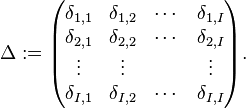
\includegraphics[width=2in]{1.png}
    \end{center}
\end{figure}  
The goal of MDS is to find  vectors x1, ...., xI such that
\begin{figure}[h]
    \begin{center}
        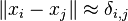
\includegraphics[width=1in]{2.png}
    \end{center}
\end{figure} 
\end{frame}



 \subsection{Procedure}
\begin{frame}
       \frametitle{Procedure}
There are several steps in conducting MDS research:
    \begin{enumerate}
        \item Formulating the problem
        \item Obtaining input data 
        \item Running the MDS statistical program
        \item Decide number of dimensions
        \item Mapping the results and defining the dimensions
        \item Test the results for reliability and validity
       \item Report the results comprehensively 
     \end{enumerate}
\end{frame}

 



\section{Applications}
\subsection{Applications}
\begin{frame}
    \frametitle{Applications}
  Applications include scientific visualisation and data mining in fields such as cognitive science, information science, psychophysics, psychometrics, marketing and ecology. 


\end{frame}




\end{document}
